%
% Main document
% ===========================================================================
% This is part of the document "Project documentation template".
% Authors: aescd5,knece1
%

%---------------------------------------------------------------------------
\documentclass[
	a4paper,					% paper format
	10pt,							% fontsize
	%twoside,					% double-sided
	%openright,				% begin new chapter on right side
	notitlepage,			% use no standard title page
	parskip=half,			% set paragraph skip to half of a line
]{scrreprt}					% KOMA-script report
%---------------------------------------------------------------------------

\raggedbottom
\KOMAoptions{cleardoublepage=plain}			% Add header and footer on blank pages


% Load Standard Packages:
%---------------------------------------------------------------------------
\usepackage[standard-baselineskips]{cmbright}

\usepackage[ngerman]{babel}										% german hyphenation
%\usepackage[latin1]{inputenc}  							% Unix/Linux - load extended character set (ISO 8859-1)
\usepackage[ansinew]{inputenc}  							% Windows - load extended character set (ISO 8859-1)
\usepackage[T1]{fontenc}											% hyphenation of words with �,� and �
\usepackage{textcomp}													% additional symbols
\usepackage{ae}																% better resolution of Type1-Fonts 
\usepackage{fancyhdr}													% simple manipulation of header and footer 
\usepackage{etoolbox}													% color manipulation of header and footer
\usepackage{graphicx}                      		% integration of images
\usepackage{float}														% floating objects
\usepackage{caption}													% for captions of figures and tables
\usepackage{booktabs}													% package for nicer tables
\usepackage{tocvsec2}													% provides means of controlling the sectional numbering
%---------------------------------------------------------------------------

% Load Math Packages
%---------------------------------------------------------------------------
\usepackage{amsmath}                    	   	% various features to facilitate writing math formulas
\usepackage{amsthm}                       	 	% enhanced version of latex's newtheorem
\usepackage{amsfonts}                      		% set of miscellaneous TeX fonts that augment the standard CM
\usepackage{amssymb}													% mathematical special characters
\usepackage{exscale}													% mathematical size corresponds to textsize
%---------------------------------------------------------------------------

% Package to facilitate placement of boxes at absolute positions
%---------------------------------------------------------------------------
\usepackage[absolute]{textpos}
\setlength{\TPHorizModule}{1mm}
\setlength{\TPVertModule}{1mm}
%---------------------------------------------------------------------------					
			
% Definition of Colors
%---------------------------------------------------------------------------
\RequirePackage{color}                          % Color (not xcolor!)
\definecolor{linkblue}{rgb}{0,0,0.8}            % Standard
\definecolor{darkblue}{rgb}{0,0.08,0.45}        % Dark blue
\definecolor{bfhgrey}{rgb}{0.41,0.49,0.57}      % BFH grey
%\definecolor{linkcolor}{rgb}{0,0,0.8}     			% Blue for the web- and cd-version!
\definecolor{linkcolor}{rgb}{0,0,0}        			% Black for the print-version!
%---------------------------------------------------------------------------

% Hyperref Package (Create links in a pdf)
%---------------------------------------------------------------------------
\usepackage[
	pdftex,ngerman,bookmarks,plainpages=false,pdfpagelabels,
	backref = {false},										% No index backreference
	colorlinks = {true},                  % Color links in a PDF
	hypertexnames = {true},               % no failures "same page(i)"
	bookmarksopen = {true},               % opens the bar on the left side
	bookmarksopenlevel = {0},             % depth of opened bookmarks
	pdftitle = {Template f�r Bachelor Thesis},	   	% PDF-property
	pdfauthor = {brd3},        					  % PDF-property
	pdfsubject = {LaTeX Template},        % PDF-property
	linkcolor = {linkcolor},              % Color of Links
	citecolor = {linkcolor},              % Color of Cite-Links
	urlcolor = {linkcolor},               % Color of URLs
]{hyperref}
%---------------------------------------------------------------------------

% Set up page dimension
%---------------------------------------------------------------------------
\usepackage{geometry}
\geometry{
	a4paper,
	left=28mm,
	right=15mm,
	top=30mm,
	headheight=20mm,
	headsep=10mm,
	textheight=242mm,
	footskip=15mm
}
%---------------------------------------------------------------------------

% Makeindex Package
%---------------------------------------------------------------------------
\usepackage{makeidx}                         		% To produce index
\makeindex                                    	% Index-Initialisation
%---------------------------------------------------------------------------
% Glossary Package
%---------------------------------------------------------------------------
% the glossaries package uses makeindex
% if you use TeXnicCenter do the following steps:
%  - Goto "Ausgabeprofile definieren" (ctrl + F7)
%  - Select the profile "LaTeX => PDF"
%  - Add in register "Nachbearbeitung" a new "Postprozessoren" point named Glossar
%  - Select makeindex.exe in the field "Anwendung" ( ..\MiKTeX x.x\miktex\bin\makeindex.exe )
%  - Add this [ -s "%tm.ist" -t "%tm.glg" -o "%tm.gls" "%tm.glo" ] in the field "Argumente"
%
% for futher informations go to http://ewus.de/tipp-1029.html
%---------------------------------------------------------------------------
\usepackage[nonumberlist]{glossaries}
\makeglossaries

\newglossaryentry{BibTeX}{name={BibTeX},description={Programm zur Erstellung von Literaturangaben und -verzeichnissen in \TeX- oder \LaTeX-Dokumenten}}
\newglossaryentry{StwVrz}{name={Stichwortverzeichnis},description={Verzeichnis mit Stichworten aus dem Text}}



%---------------------------------------------------------------------------

% Intro:
%---------------------------------------------------------------------------
\begin{document}                              	% Start Document
\settocdepth{section}														% Set depth of toc
\pagenumbering{roman}														
%---------------------------------------------------------------------------

\providecommand{\titel}{Intégration continues}					% Titel der Arbeit aus Datei titel.tex lesen
\providecommand{\versionnumber}{1.2}			%  Hier die aktuelle Versionsnummer eingeben
\providecommand{\versiondate}{01.02.2014}		%  Hier das Datum der aktuellen Version eingeben				% Versionsnummer und -datum aus Datei version.tex lesen

% Set up header and footer
%---------------------------------------------------------------------------
\makeatletter
\patchcmd{\@fancyhead}{\rlap}{\color{bfhgrey}\rlap}{}{}		% new color of header
\patchcmd{\@fancyfoot}{\rlap}{\color{bfhgrey}\rlap}{}{}		% new color of footer
\makeatother

\fancyhf{}																		% clean all fields
\fancypagestyle{plain}{												% new definition of plain style	
	\fancyfoot[OR,EL]{\footnotesize \thepage} 	% footer right part --> page number
	\fancyfoot[OL,ER]{\footnotesize \titel, Version \versionnumber, \versiondate}	% footer even page left part 
}

\renewcommand{\chaptermark}[1]{\markboth{\thechapter.  #1}{}}
\renewcommand{\headrulewidth}{0pt}				% no header stripline
\renewcommand{\footrulewidth}{0pt} 				% no bottom stripline

\pagestyle{plain}
%---------------------------------------------------------------------------


% Title Page and Abstract
%---------------------------------------------------------------------------
%%
% Project documentation template
% ===========================================================================
% This is part of the document "Project documentation template".
% Authors: brd3, kaa1
%

\begin{titlepage}


% BFH-Logo absolute placed at (28,12) on A4 
% Actually not a realy satisfactory solution but working.
%---------------------------------------------------------------------------
\setlength{\unitlength}{1mm}
\begin{textblock}{20}[0,0](28,12)
	
\includegraphics[scale=1.0]{bilder/BFH_Logo_B.png}
\end{textblock}
\color{black}

% Institution / Titel / Untertitel / Autoren / Experten:
%---------------------------------------------------------------------------
\begin{flushleft}

\vspace*{21mm}

\fontsize{26pt}{40pt}\selectfont 
\titel 				\\							% Titel aus der Datei vorspann/titel.tex lesen
\vspace{2mm}

\fontsize{16pt}{24pt}\selectfont\vspace{0.3em}
Hier steht ein Untertitel 			\\							% Untertitel eingeben
\vspace{5mm}

\fontsize{10pt}{12pt}\selectfont
\textbf{Art der Arbeit (Semesterarbeit / Bachelorthesis / etc.)} \\									% eingeben
\vspace{7mm}

% Abstract (eingeben):
%---------------------------------------------------------------------------
\begin{textblock}{150}(28,100)
\fontsize{10pt}{12pt}\selectfont
[Kurztext (Abstract) einf�gen, falls gew�nscht] \\ 
Dieses Dokument dient als Vorlage f�r die Erstellung von Berichten nach den Richtlinien der BFH. Die Vorlage ist in \LaTeX{} erstellt und unterst�tzt das automatische Erstellen von diversen Verzeichnissen, Literaturangaben, Indexierung und Glossaren. Dieser kleine Text ist eine Zusammenfassung �ber das vorliegenden Dokument mit einer L�nge von 4 bis max. 8 Zeilen. \\
Das Titelbild kann in den Zeilen 157/158 der Datei template.tex ein- oder ausgeschaltet werden.
\end{textblock}

\begin{textblock}{150}(28,225)
\fontsize{10pt}{17pt}\selectfont
\begin{tabbing}
xxxxxxxxxxxxxxx\=xxxxxxxxxxxxxxxxxxxxxxxxxxxxxxxxxxxxxxxxxxxxxxx \kill
Studiengang:	\> [z.B. Elektro- und Kommunikationstechnik]	\\			% Namen eingeben
Autoren:		\> [Test Peter, M�ster R�s�]		\\					% Namen eingeben
Betreuer:	\> [Dr.~Xxxx Xxxx, Dr.~Yyyy Yyyy]		\\					% Namen eingeben
Auftraggeber:	\> [Wwwww AG]						\\					% Namen eingeben
Experten:		\> [Dr.~Zzzz Zzzz]				\\					% Namen eingeben
Datum:			\> \versiondate					\\		% aus Datei vorspann/version.tex lesen
\end{tabbing}

\end{textblock}
\end{flushleft}

\begin{textblock}{150}(28,280)
\noindent 
\color{bfhgrey}\fontsize{9pt}{10pt}\selectfont
Berner Fachhochschule | Haute �cole sp�cialis�e bernoise | Bern University of Applied Sciences
\color{black}\selectfont
\end{textblock}


\end{titlepage}

%
% ===========================================================================
% EOF
%
		% activate for Titelseite ohne Bild
%
% Project documentation template
% ===========================================================================
% This is part of the document "Project documentation template".
% Authors: brd3, kaa1
%

\begin{titlepage}


% BFH-Logo absolute placed at (28,12) on A4 and picture (16:9 or 15cm x 8.5cm)
% Actually not a realy satisfactory solution but working.
%---------------------------------------------------------------------------
\setlength{\unitlength}{1mm}
\begin{textblock}{20}[0,0](28,12)
	
\includegraphics[scale=1.0]{bilder/BFH_Logo_B.png}
\end{textblock}

\begin{textblock}{154}(28,48)
	\begin{picture}(150,2)
		\put(0,0){\color{bfhgrey}\rule{150mm}{2mm}}
	\end{picture}
\end{textblock}

\begin{textblock}{154}[0,0](28,50)
	
\includegraphics[scale=0.6]{bilder/CI_titleImage.png}			% Titelbild definieren
\end{textblock}

\begin{textblock}{154}(28,135)
	\begin{picture}(150,2)
		\put(0,0){\color{bfhgrey}\rule{150mm}{2mm}}
	\end{picture}
\end{textblock}
\color{black}

% Institution / Titel / Untertitel / Autoren / Experten:
%---------------------------------------------------------------------------
\begin{flushleft}

\vspace*{115mm}

\fontsize{26pt}{28pt}\selectfont 
\titel 				\\							% Titel aus der Datei vorspann/titel.tex lesen
\vspace{2mm}

\fontsize{10pt}{12pt}\selectfont
\textbf{Rapport 2 - Séminaire Info 2016} \\									% eingeben
\vspace{3mm}

\begin{textblock}{150}(28,225)
\fontsize{10pt}{17pt}\selectfont
\begin{tabbing}
xxxxxxxxxxxxxxx\=xxxxxxxxxxxxxxxxxxxxxxxxxxxxxxxxxxxxxxxxxxxxxxx \kill
Filière d'études:	\> Informatique	\\			% Namen eingeben
Auteurs:		\> Emanuel Knecht, David Aeschlimann		\\					% Namen eingeben
Conseiller:	\> 		Dr. Bernhard Anrig		\\					% Namen eingeben
Date:			\> \versiondate					\\		% aus Datei vorspann/version.tex lesen
\end{tabbing}

\end{textblock}
\end{flushleft}

\begin{textblock}{150}(28,280)
\noindent 
\color{bfhgrey}\fontsize{9pt}{10pt}\selectfont
Berner Fachhochschule | Haute école spécialisée bernoise | Bern University of Applied Sciences
\color{black}\selectfont
\end{textblock}


\end{titlepage}

%
% ===========================================================================
% EOF
%
			% activate for Titelseite mit Bild
%---------------------------------------------------------------------------

% Table of contents
%---------------------------------------------------------------------------
\tableofcontents
%\cleardoublepage
%---------------------------------------------------------------------------

% Main part:
%---------------------------------------------------------------------------
\pagenumbering{arabic}

\chapter{Einleitung}
\label{chap:einleitung}

Dieses Dokument ist der schriftliche Teil des Informatikseminars an der Berner Fachhochschule. In den kommenden Kapiteln wird die Aspektorientierte Programmierung mit AspectJ vorgestellt und erkl�rt.

\nocite{laddad:aspectj}

\section{Auftrag}
\label{sec:einleitung_auftrag}



\section{Vorgehen}
\label{sec:einleitung_vorgehen}


\chapter{Aspektorientierte Programmierung}
\label{chap:aop}

\section{Geschichte}
\label{sec:aop_geschichte}

Das Konzept der Aspektorientierten Programmierung wurde im Xerox PARC (Palo Alto Research Center Incorporated) entwickelt und gewann ab 1995 an Wichtigkeit. Wie bei allen neuen Spezifikationen war der Umfang und die Bestandteile der Aspektorientierten Programmierung zunächst nicht klar abgegrenzt. Gregor Kiczales und ein Team von Forschern waren massgeblich an der Entwicklung von AOP beteiligt.\\
Nach Entwicklung des theoretischen Grundlage folgte im Jahre 1998 eine erste Version von AspectJ, eine Implementation von AOP in Java. Die Version 1.0 von AspectJ wurde jedoch erst im Jahre 2002 nach weiterer Forschung veröffentlicht.\footnote{\cite{lopes:historyaop}} \\
Das Konzept der Aspektorientierte Programmierung wurde durch die Publikation von AspectJ bekannt und es wurden seither Erweiterungen für die meisten populären Programmiersprachen entwickelt und veröffentlicht. 

Die Entwicklung und der Betrieb von AspectJ wurde von XeroX Parc an Eclipse weitergereicht. Dort läuft AspectJ bis heute als Open-Source Projekt weiter. Mit der Version 1.8.7 wurde am 9. September 2015 die bis heute aktuellste Version von AspectJ veröffentlicht.

\section{Motivation}
\label{sec:aop_motivation}

Einer der Hauptgründe warum AOP entwickelt wurde ist die erweiterte Modularität, welche damit erreicht werden kann. Beim Design eines Systems werden in der Regel verschiedene Kategorien von Funktionalitäten aufgestellt und so die Software in verschiedene sogenannte Anliegen (concerns) aufgeteilt. Diese Anliegen werden isoliert betrachtet und der Funktionsumfang einzeln spezifiziert. Dabei unterscheidet man zwischen den folgenden zwei Gruppen von Anliegen einer Applikation:

\begin{itemize}
	\item Core concerns (Kernanliegen)\\
	Hierbei handelt sich um die Kernfunktionalität der Applikation, die sogenannte Business Logic. Diese Gruppe beinhaltet zum Beispiel den Datenbankzugriff sowie die Interaktion mit dem Benutzer
	\item Cross-cutting concerns (System-übergreifende Anliegen) \\
	Andere Funktionalitäten wie das Logging, die Sicherheit, Concurrency sowie Transaktionen betreffen das gesamte System und werden an vielen verschiedenen Orten in der Business Logic verwendet.
\end{itemize}

Diese Gruppierung dient als Grundlage zur Veranschaulichung, warum gerade bei der Modularisierung die OOP Schwachstellen aufweist.\newpage

\subsection{Objektoriente Programmierung}
\label{sec:aop_oop}

Mit der Objektorientierten Programmierung wurden viele Probleme und Unschönheiten von Prozeduralen Sprachen gelöst. Die OOP vereinfacht und abstrahiert die Softwareentwicklung. Einige der wichtigsten Konzepte der OOP sind:

\begin{itemize}
	\item Encapsulation: Daten und Methoden zur Veränderung derjenigen werden in Objekten gekapselt
	\item Inheritance: Das Verhalten oder die Daten können von einer Klasse geerbt werden.
	\item Polymorphism: Verschiedene Objekte mit gleichem Supertyp reagieren unterschiedlich bei einem Methodenaufruf. Der genaue Typ des aufgerufenen Objektes soll der aufrufenden Instanz nicht bekannt sein
\end{itemize}

Die OOP erlaubt es Code modular zu strukturieren und Daten zu kapseln. Mit steigender Komplexität wird es jedoch schwierig den Code klar zu trennen und die Abhängigkeiten zwischen Modulen so klein wie möglich zu halten.\\

Die Kernanliegen der Applikation werden in Klassen der Business Logic abgebildet. Diese Klassen werden jedoch sehr schnell durch den Code der System-übergreifenden Anliegen "verschmutzt". Dadurch wird das Single Responsibility Principle verletzt; eine Klasse ist nicht nur für ein bestimmtes Anliegen verantwortlich. Die folgende Graphik zeigt eine solche Beispielklasse, welche das beschriebene Phänomen veranschaulichen soll. Nur ein kleiner Teil der Methode (rot markiert) beschäftigt sich mit der Ausführung des Kernanliegens dieser Klasse, der Rest mit den System übergreifenden Anliegen.

\begin{figure}[H]
	\centering
		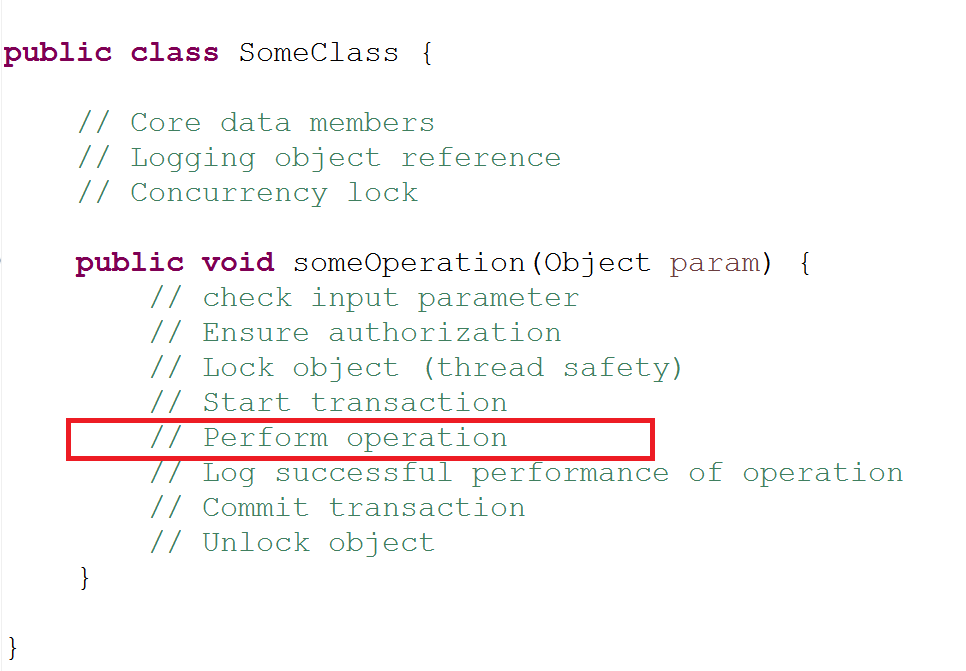
\includegraphics[scale=1.0]{bilder/motivationprogram}
	\caption{Beispielsklasse - Motivation für AOP}
	\label{fig:classmotivationaop}
\end{figure}



\paragraph{Code Tangling}

Von Code Tangling (to tangle - sich verwickeln) spricht man wenn ein Modul verschiedene Anliegen bearbeitet. Als Beispiel kann man die Abbildung \ref{fig:classmotivationaop} nehmen. Während der Designphase werden alle Anliegen seperat entworfen und in der Implementation wird dennoch alles wieder miteinander verwickelt und verwoben. Die gewünschte Trennung der Anliegen und Modularisierung der Applikation wird mit OOP nicht vollständig erreicht.

\paragraph{Code Scattering}

Bei Code Scattering (to scatter - streuen) ist die Perspektive eine andere. Die Funktionen eines Moduls werden in verschiedene anderen Modulen verwendet und so im ganzen System gestreut. Es gibt oftmals verschiedene Arten um auf Funktionen eines Modules zuzugreifen. Durch diese Aufrufe wird ein Teil der Logik des aufzurufenden Moduls ins aufrufende Modul verschoben. Folgende Abbildung soll dies anhand eines Sicherheitsmoduls veranschaulichen.

\begin{figure}[H]
	\centering
		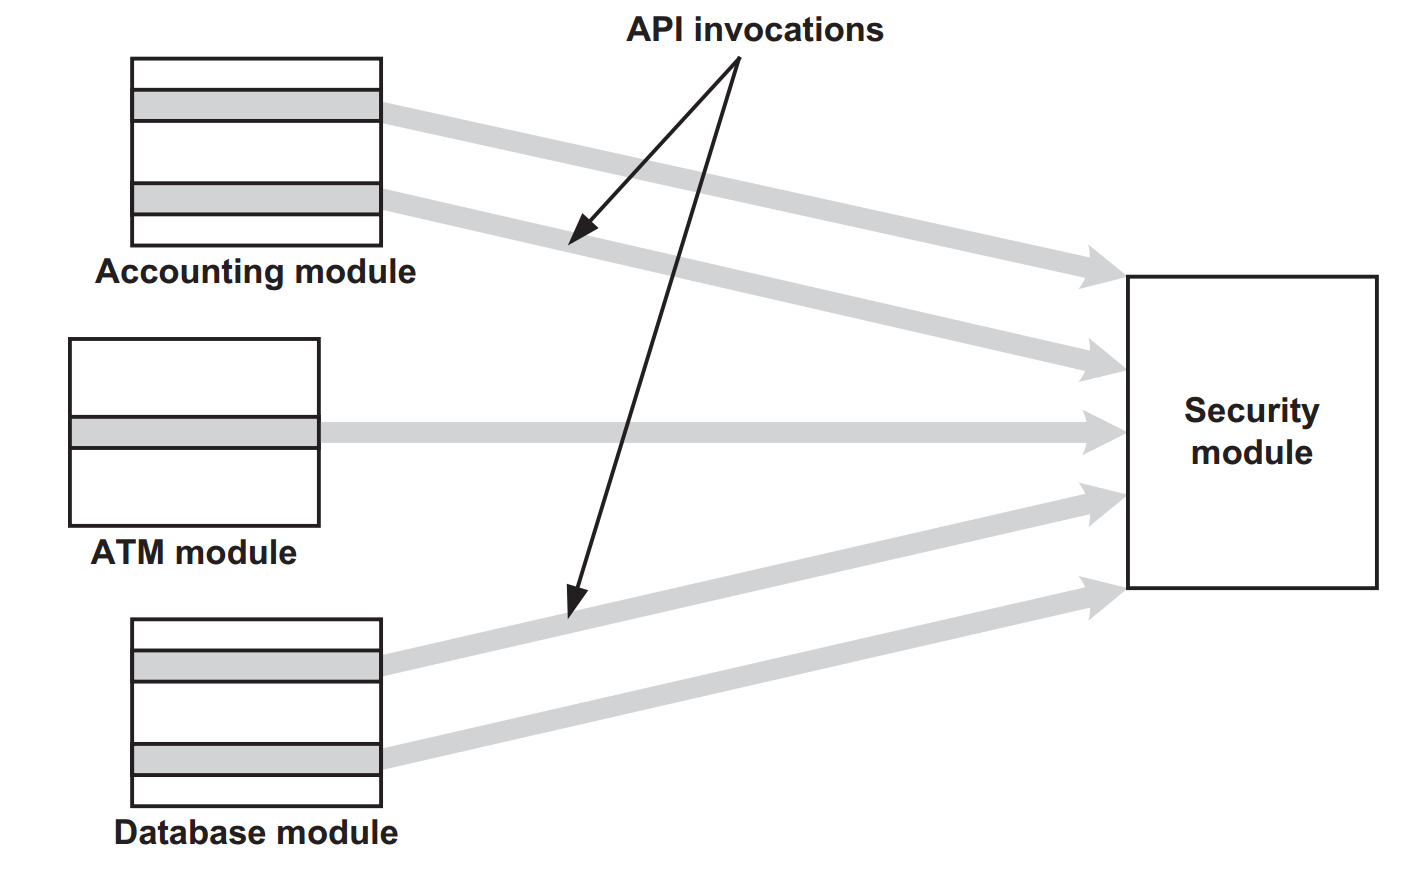
\includegraphics[scale=0.5]{bilder/motivationsCodeScattering}
	\caption{Code Scattering (\cite[p~54]{laddad:aspectj})}
	\label{fig:motivationcs}
\end{figure}

Bei Verwendung von OOP ist das Code Tangling und Code Scattering unumgänglich. Selbst bei einem perfekt designten System werden diese Phänomene vorhanden sein. Dies beeinflusst Software Design und Entwicklung auf vielerlei Arten: Schlechte Nachvollziehbarkeit, weniger Produktivität, weniger Wiederverwendbarkeit von Code, viele repetitive Arbeiten, schlechtere Qualität und Wartbarkeit von Applikationen. Aus diesen Gründen macht es Sinn nach Alternativen zu OOP zu suchen, ohne jedoch auf deren Vorzüge zu verzichten.

\subsection{Modularisierung mit AOP}
\label{sec:aop_modaop}
AOP ist diese Alternative. Bleiben wir beim Beispiel eines Security Moduls; Das Modul wird mit Klassen implementiert und mittels Interfaces gegen aussen sichtbar gemacht. In der OOP werden nun alle Codeteile welche Securityfunktionen verwenden möchten einen Aufruf dieses Moduls beinhalten. Bei einer Änderung in der API müssen unter Umständen tausende Aufrufe ebenfalls geändert werden. Mit AOP jedoch beinhalten die Client Module keine Aufrufe mehr. Aufrufe des Sicherheitsmoduls werden bei genau definierten Punkten im Code automatisch ausgelöst. Es kann beispielsweise definiert werden, dass bei allen öffentlichen Methoden einer Klasse vor Ausführung des Bodys die Berechtigung des Benutzers geprüft wird. Bei dieser Deklaration der Einstiegspunkte im Code und des in diesen Fällen auszuführenden Codes spricht man von einem Aspect. Um diese automatische Ausführung möglich zu machen muss der Code der Kernanliegen (Business Logic) mit dem des Aspects verwebt werden. Man spricht hierbei von Weaving.
\begin{figure}[H]
	\centering
		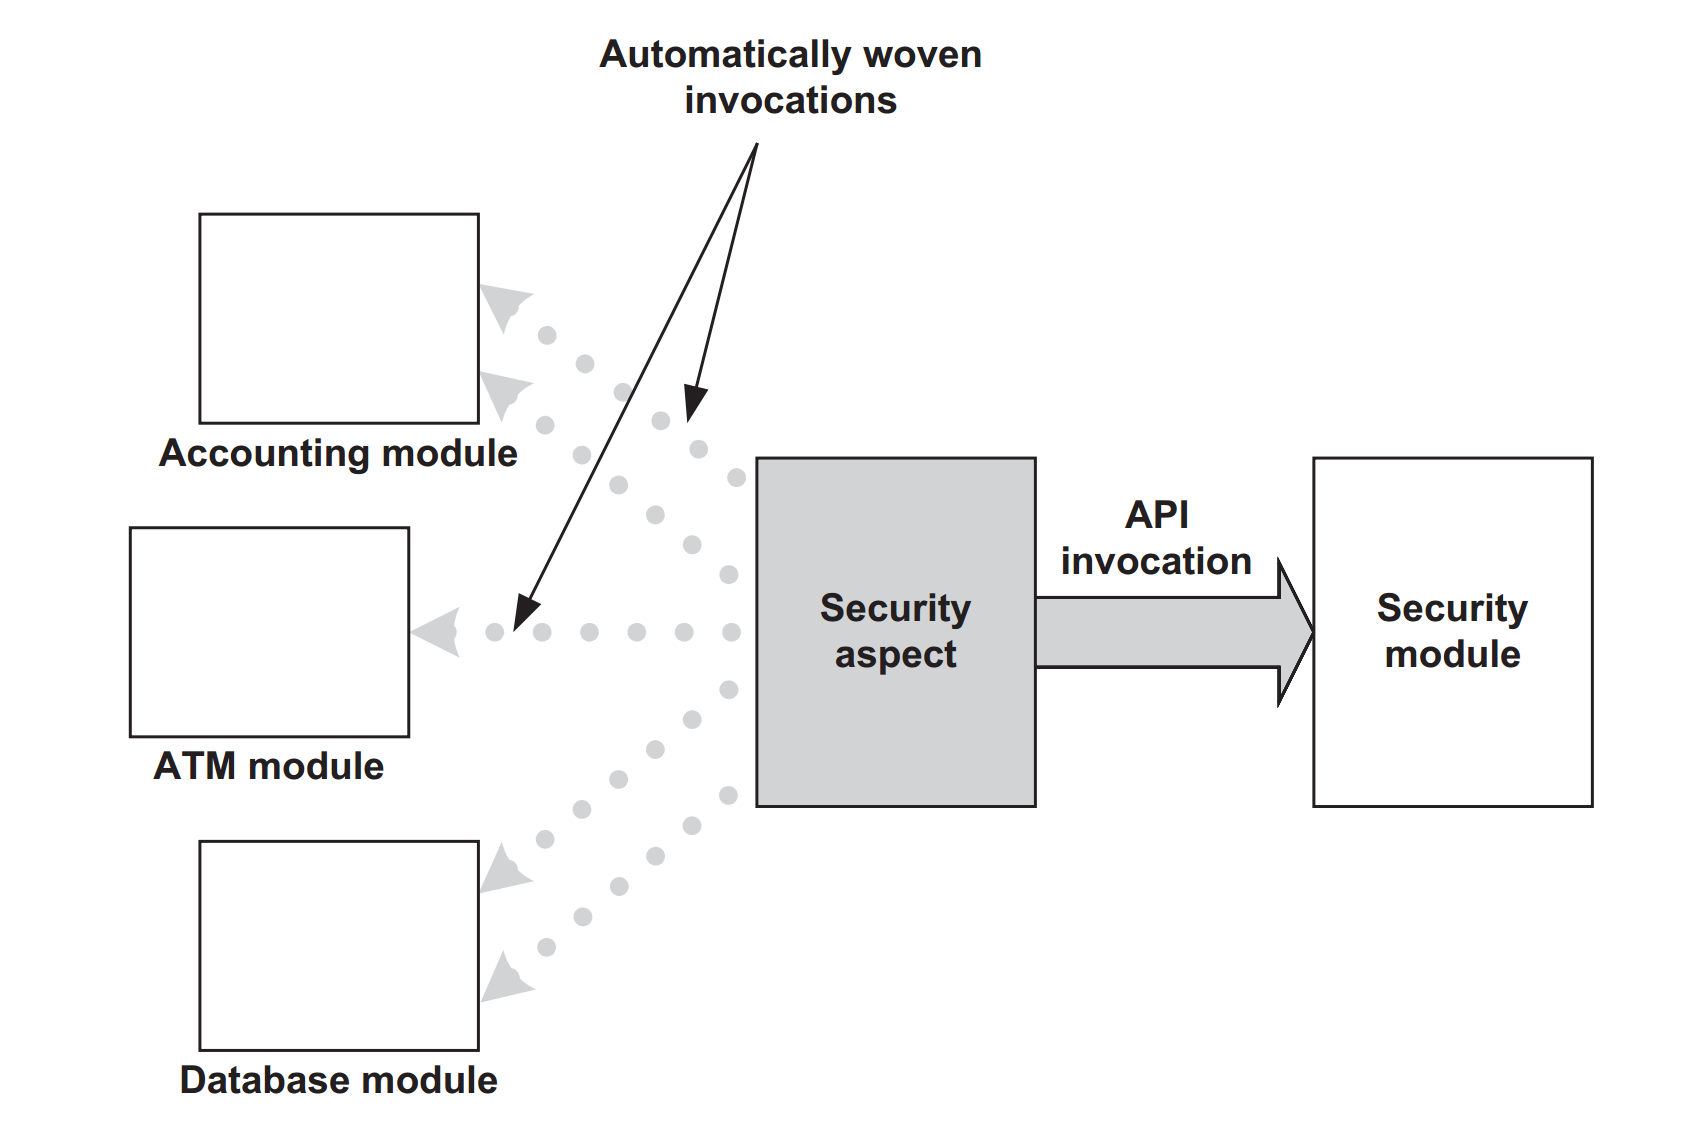
\includegraphics[scale=0.5]{bilder/motivationAop}
	\caption{Systemdesign mit AOP (\cite[p~55]{laddad:aspectj})}
	\label{fig:motivationaop}
\end{figure}

\section{Aspektorientierte Sprache}
\label{sec:aop_lang}
Die Aspektorientierte Programmierung ist eine Methode der Softwareentwicklung. Damit eine Programmiersprache um den Funktionsumfang von AOP erweitert werden kann, muss zuerst ein genaues Konzept der verschiedenen Komponenten einer Aspektorientierten Programmiersprache spezifiziert und diese Spezifikation anschliessend umgesetzt werden.
\subsection{Spezifikation}
\subparagraph{Programmiersprache}
Als Grundlage für die Entwicklung eines Aspektorientierten Programms dient eine Programmiersprache. Es werden in der Regel bestehende Programmiersprachen wie C, C++, CSharp und Java verwendet, da diese von vielen Entwicklern bereits verstanden und angewendet werden. Im Falle der Entwicklung einer neuen Applikation werden alle Module in jener Programmiersprache isoliert voneinander entwickelt.
\subparagraph{Weaving Rules Spezifizierung}
Die Sprache muss nun eine Möglichkeit bieten um diese entwickelten Module miteinander verknüpfen zu können. Dazu müssen sogenannte Weaving Rules deklariert werden. Die Weaving Rules bestimmen wie der Code verknüpft wird. Hierfür können Standardelemente einer Sprache verwendet (Annotations, Xml config) oder auch die bestehende Sprache um neue Bestandteile erweitert werden (Keywords).
\subsection{Implementation}
Eine Implementation einer AOP Sprache kann in zwei Schritte gegliedert werden. Zuerst muss die Verknüpfung der verschiedenen Anliegen mittels Weaving rules sichergestellt und anschliessend daraus  ausführbarer Code generiert werden. Bei AOP führt der sogenannte \textbf{Weaver} diese Aufgaben aus. Es gibt drei verschiedene Typen von Weavern:

\begin{itemize}
\item Source-to-Source weaver \\ Der Sourcecode der Core und Crosscutting concerns wird zuerst verwoben und dieser neu entstandene Source Code von einem regulären Compiler kompiliert. 
\item Binary weaver \\ Der Sourcecode der Core und Crosscutting concerns wird zuerst kompiliert und der daraus entstandene Byte Code wird vom Weaver verknüpft.
\item Load time weaver \\ Vergleichbar mit dem Byte Code weaving, ausser dass der Verknüpfungsvorgang erst beim Aufrufen des Programms statt findet.
\end{itemize}

Ein Weaver ist nicht mit einem Compiler gleichzustellen. Je nach Typus braucht es jedoch eine enge Zusammenarbeit zwischen Weaver und Compiler. Deswegen stellen einige Anbieter von AOP Erweiterungen den Entwicklern ihre eigenen Compiler inklusive Weaver zur Verfügung.\newpage

\section{Konzepte}
\label{sec:aop_concepts}

Die folgenden Konzepte sind die Grundlage von Aspekorientierter Programmierung. Dies ist ein generisches Modell und nicht jede Implementation einer Aspekorientierten Programmiersprache muss zwingend alle Konzepte implementieren. AspectJ jedoch implementiert alle hier vorgestellten Komponenten.\footnote{\cite[p~58]{laddad:aspectj}}

\begin{itemize}
\item \textit{Identifizierbare Punkte in der Ausführung des Programms} \\ Während der Ausführung eines Programms gibt es Points of Interest. Solche Punkte sind beispielsweise der Aufruf einer Methode oder das Werfen von Exceptions. Im Umfeld von AOP werden diese Punkte \textbf{Join Points} genannt. 
\item \textit{Selektion von Punkten während des Programmablaufs}\\ Diese Join Points müssen irgendwie angesteuert werden können. Dies geschieht mit einem \textbf{Pointcut}. Ein Pointcut beinhaltet ein Statement, welches eine gewisse Anzahl von Join Points selektiert. So könnten beispielsweise alle öffentlichen Methoden aller Klassen eines Moduls selektiert werden. Ein Pointcut kann auch auf den Kontext eines Join Points zugreifen (Parameter einer Methode, Typ, Klasse etc.).
\item \textit{Veränderung des regulären Programmablaufs (dynamic crosscutting)}\\
Wenn ein Join Point von einem Pointcut selektiert wurde, soll der reguläre Programmablauf durch Ausführung von zusätzlichem Code verändert werden. Dieser Code ist vom Entwickler frei wählbar und der Programmablauf wird dadurch dynamisch. Der auszuführende Code wird in einem \textbf{Advice} gesammelt.
\item \textit{Veränderung der statischen Struktur des Systems (static crosscutting)}\\
Um gewisse crosscutting concerns umsetzen zu können müssen in einer Klasse zusätzliche Felder deklariert werden (\textbf{inter-type declaration}). Ausserdem kann es nötig sein bereits beim weaving zu wissen, ob gewisse Join Points im System vorhanden sein werden, um angemessen darauf reagieren zu können. Dies wird durch \textbf{weave-time declarations} ermöglicht.

\item \textit{Deklaration aller Konstrukte}\\
All diese Komponenten (pointcuts, dynamic \& static crosscutting) werden logisch an einem Ort, dem \textbf{Aspect}, deklariert. Der Aspekt kapselt ein systemübergreifendes Anliegen, respektive enthält die Verknüpfung zwischen der Business Logic und einem systemübergreifenden Modul. 
\end{itemize}

Alle diese Konzepte werden in der Abbildung \ref{fig:concepts} zusammengefasst und deren Beziehung zueinander graphisch abgebildet.

\begin{figure}[H]
	\centering
		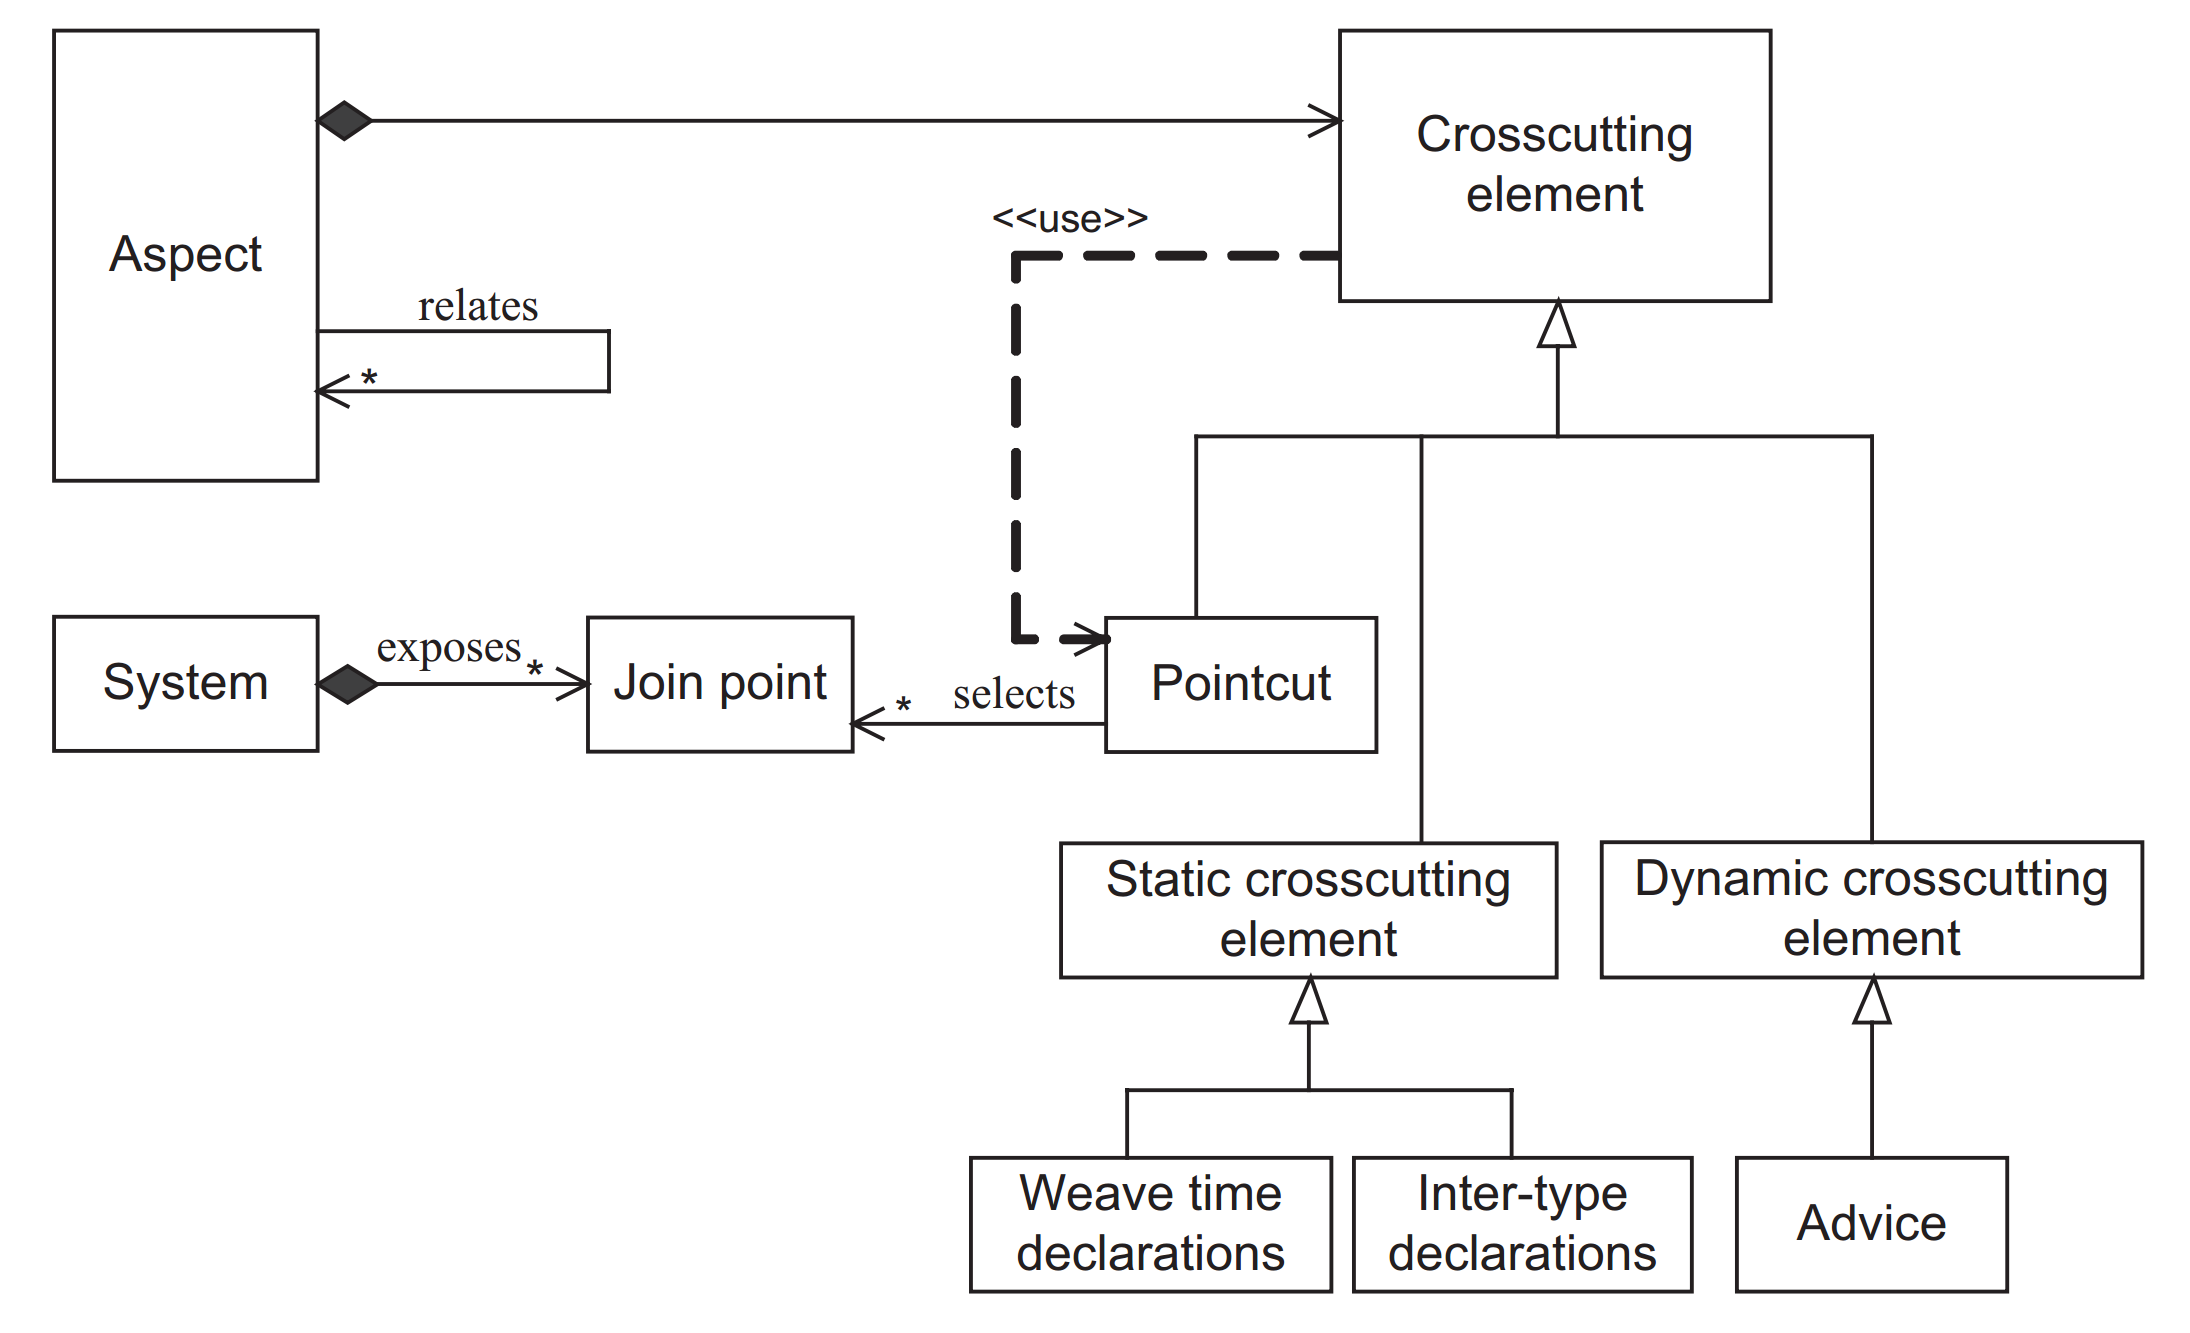
\includegraphics[scale=0.5]{bilder/concepts}
	\caption{AOP Konzepte (\cite[p~60]{laddad:aspectj})}
	\label{fig:concepts}
\end{figure}
\newpage

\section{Programmiersprachen}

Beinahe für jede bekanntere Programmiersprache gibt es eine Erweiterung oder ein Framework um AOP als Gesamtes oder Teile davon zu ermöglichen. Nachfolgend eine Übersicht über die bekanntesten Sprachen mit den verbreitesten Frameworks.

\subsection{Java}

AspectJ gilt als erstes komplettes AOP Framework überhaupt und ist deshalb auch am Verbreitesten.

\begin{itemize}
\item AspectJ - Wird detailliert im Kapitel \nameref{chap:aspectj} beleuchtet
\item Spring AOP - Spring ist ein Framework zur Entwicklung von Java Applications. Auch dort gibt es die Möglichkeit AOP zu verwenden. Jedoch ist man limitiert auf Methodenaufrufe als Join Points.
\end{itemize}

\subsection{C, C++}

\begin{itemize}
\item AspectC++ - Eine Adaptierung von AspectJ in C/C++ \footnote{\cite{net:aspectc}}
\end{itemize}

\subsection{.NET Framework}

CSharp unterstützt nativ sogenannte Extension methods. Hiermit können nachträglich zu Klassen oder Interfaces Methoden hinzugefügt werden (static crosscutting). Dies ist allerdings nur ein Teil der AOP, für alles andere benötigt man ein Framework.

\begin{itemize}
\item PostSharp - Kommerzielle Software welche eine grosse Verbreitung geniesst (Siemens, Roche, Lufthansa und viele mehr) \footnote{\cite{net:postsharp}}
\item AspectSharp - AOP Framework für .NET\footnote{\cite{net:aspectsharp}}
\item Afterthought - Afterthought ist eine Open Source Alternative zu Postsharp.\footnote{\cite{net:afterthought}}
\end{itemize}

\subsection{Nemerle}
Nemerle ist eine relativ junge, quelloffene Programmiersprache (2003 erstmals öffentlich erschienen, erster stabiler Release 13. Mai 2011). Sie benutzt die Common Language Infrastucture (CLI) und kann somit Plattformunabhängig (.net/Mono) genutzt werden. 
Nemerle unterstützt Funktionale-, Objektorientierte- und Imperative Programmierung und verfügt über ein mächtiges Meta-Programming System (Makros) welches dadurch auch Aspektorientierte Programmierung ermöglicht. Beispiele unter: \citet{github:nemerleaopsrc}
\chapter{AspectJ}
\label{chap:aspectj}
\section{Bestandteile von AspectJ}
In diesem Kapitel betrachten wir, wie die verschiedenen Komponenten des im Abschnitt \nameref{sec:aop_concepts} vorgestellten Modells einer Aspektorientierten Programmiersprache in AspectJ umgesetzt sind. Alle hier verwendeten Codeteile sind Bestandteil unseres Demoprogrammes, welches sich im Anhang befindet (\nameref{chap:demoprogramm}).

\subsection{Allgemein}
\subsubsection{Aspect}
Der Aspect ist die zentrale Einheit in AspectJ. Im Aspect werden alle Bestandteile eines Anliegens einer Applikation zusammengefasst. Ein Aspect kann gleich wie eine normale Javaklasse Attribute und Methoden enthalten und dient zur Kapselung des Anliegens. So werden alle Funktionen welche das Logging einer Applikation betreffen im Logging Aspect zusammengefasst. Aspects werden in Dateien mit der Endung .aj gespeichert.

\lstinputlisting[language=Java, firstline=3, lastline=9]{../src/AspectJDemo/src/ch/bfh/infsem/aspectjdemo/LogAspectShort.aj}
\subsubsection{Join-Point Modell}
Die Join Points sind die Punkte im Programmablauf, wo die Systemübergreifenden Anliegen im Code der Business Logic anknüpfen können. AspectJ bietet eine Menge solcher Punkte an und der Entwickler muss sich genau überlegen welchen Punkt er als Einstiegspunkt verwenden will, da der Kontext des Join Points sich teils sehr stark unterscheidet (Bsp. Aufruf oder Ausführung von Methode). Die nachfolgende Tabelle zeigt eine Übersicht der vorhandenen Join Points in AspectJ.

\begin{table}[H]
	\centering
		\begin{tabular}{p{0.30\textwidth} p{0.65\textwidth}} \toprule
			\textbf{Kategorie} & \textbf{Join Point} \\ \midrule
			Methode & Ausführung der Methode (Method Body) \\ \midrule
			Methode & Aufruf der Methode (aufrufender Kontext) \\ \midrule
			Konstruktor & Ausführung des Konstruktors \\ \midrule
			Konstruktor & Aufruf des Konstruktors \\ \midrule
			Feldzugriff & Lesender Zugriff auf Feld \\ \midrule
			Feldzugriff & Schreibender Zugriff auf Feld \\ \midrule
			Exception Handling & Catch Block \\ \midrule
			Initialisierung & Laden, Initialisierung und Pre-Init einer Klasse \\ \midrule
			Advice & Ausführung eines Advice
			 \\ \bottomrule
		\end{tabular}
	\caption{Übersicht über alle Join Points in AspectJ}
	\label{tab:overview}
\end{table}

Die Pointcuts wählen einen oder mehrere solcher Punkte aus und können intern benannt werden. Die Syntax der Pointcuts beruht auf Signaturen von Methoden oder Feldern. Die Selektion der Join Points kann aufgrund des Access Modifiers, der Rückgabetypen, der Klasse und des Namens des Members eingeschränkt werden. Der Stern kann als Wildcard Charakter verwendet werden. So selektiert der nachfolgende pointcut alle Methoden, aller Klassen die öffentlich sind.

\lstinputlisting[language=Java, firstline=11, lastline=11]{../src/AspectJDemo/src/ch/bfh/infsem/aspectjdemo/LogAspect.aj}

\subsection{Dynamic crosscutting}
Beim Dynamic crosscutting wird der Programmfluss verändert und um zusätzlichen Code erweitert. Dieser zusätzliche Code wird in AspectJ in einem Advice gekapselt. Der Advice kann vor, nach oder um den Join Point herum ausgeführt werden (before, after, around). Folgender Advice schreibt den Start und das Ende der Methode auf die Konsole. Über das Objekt thisJoinPoint kann auf den Kontext des Join Points zugegriffen werden. In diesem konkreten Fall verwenden wir den Kontext um auf die Signatur der Methode zuzugreifen.

\lstinputlisting[language=Java, firstline=13, lastline=18]{../src/AspectJDemo/src/ch/bfh/infsem/aspectjdemo/LogAspect.aj}

\subsection{Static crosscutting}

Mit Static crosscutting wird die statische Struktur des Programms verändert. Es können Members wie Variablen und Methoden zu Klassen hinzugefügt, Annotations an Typen, Feldern, Methoden und Konstruktoren angebracht, Warnings und Errors generiert und Exceptions abgefangen werden.

\paragraph{Inner-type declaration}

Mit Inter-type declarations können Variablen und Methoden an bestehende Klassen angefügt werden, auch wenn man keinen Zugrif auf deren Code hat (in APIs).\\Beispiel:\\


\begin{lstlisting}[language=Java]
public interface Visitor{
	void visitPoint(java.awt.Point p);
}

public aspect PointVisitor{
	private ArrayList<Visitor> java.awt.Point.visitors = new ArrayList<Visitor>();

	public void java.awt.Point.visit(Visitor v){
		visitors.add(v);
		v.visitPoint(this);
	}
}

//====== Call ======
public class SomeCallerClass{
	public void someMethod(Visitor v){
		java.awt.Point p = new jawa.awt.Point(0,0);
		
		p.visit(v);
	}
}
\end{lstlisting}

Hier wird der Klasse java.awt.Point eine Methode visit(Visitor) hinzugefügt, welche sich alle Besucher (visitors) dieses Punktes in einer ArrayList merkt. Mit dem Code aus dem Beispiel könnte diese Liste zwar nicht ausgelesen werden, was aber für diese Veranschaulichung keine Rolle spielt.\\
Inner-type declarations können auch verwendet werden um Standardimplementationen für Interfaces bereitzustellen.

\paragraph{Type-hierarchy modification}
Mit Aspekten kann auch die Klassenhierarchie verändert werden. Sowohl das implementieren von Interfaces als auch das Erweitern und Erben von Klassen ist möglich. Multi-inheritance wird jedoch nach wie vor nicht unterstützt.\\
Hier einige Beispiele:\\

\begin{lstlisting}[language=Java]
//====== 1 ======

public class VisitorImpl{
}

public aspect VisitorImplementationAspect{
	declare parents: VisitorImpl implements Visitor

	public void VisitorImpl.visit(Visitor v){
		void visitPoint(java.awt.Point p);
	}

}

//====== 2 ======

@interface PointVisitor{
	//Custom Annotation
}

@PointVisitor
public class PointVisitorImpl{
}

public aspect PointVisitorImplementationAspect{
	declare parents: @PointVisitor * extends VisitorImpl;
}

//====== Call ======
public class AnotherCallerClass{
	public void anotherMethod(){
		java.awt.Point p = new jawa.awt.Point(0,0);
		Visitor v1 = new VisitorImpl();
		Visitor v2 = new PointVisitorImpl();
		p.visit(v1);
		p.visit(v2);
	}
}
\end{lstlisting}

Im ersten Teil wird die Klasse VisitorImpl als Implementation von Visitor deklariert. Bekanntlich müssen bei Interfaces alle Methoden implementiert werden. Auch dies kann wie wir zuvor gesehen haben vom Aspekt übernommen werden.
Anstelle des Klassennamen kann auch ein Pattern angegeben werden, sodass mehrere Klassen aufs Mal verändert werden können. Dies ist beim zweiten Beispiel der Fall, wo alle Klassen mit der @PointVisitor Annotation zu Subklassen von VisitorImpl werden.

\paragraph{Weave-time declaration}
Weave-time declarations geben dem Entwickler die möglichkeit Errors und Warnings zu generieren. Eine typische Anwendung dafür ist es zu verhindern, dass nicht unterstützte Methoden verwendet werden.

\section{Syntaxvarianten}
Für die Verwendung von AspectJ können zwei Syntaxvarianten eingesetzt werden.

\begin{itemize}
\item Traditionelle Variante \\
Diese Variante haben wir bisher in allen unseren Beispielen verwendet. Man verwendet die Schlüsselwörter von AspectJ und der gesamte Umfang von AspectJ steht zur Verfügung. Man nennt diese Variante traditionell, da dies zu Beginn die erste und einzige Möglichkeit war um AspectJ zu verwenden.
\item Annotation-based Variante \\
In der annotation-based Variante verwendet man normale Javaobjekte um die Konstrukte von AspectJ abzubilden. Diese Klassen und Methoden werden mit Annotations versehen, damit der Weaver versteht wie der Code zu verknüpfen ist. Diese Variante wurde erst ab Version 5 von AspectJ eingeführt und es sind nicht ganz alle Konstrukte abbildbar.
\item Xml Variante\\
Wird vom Load-time Weaving-Agent verwendet um den Bytecode geladener Klassen mit jenem der Aspekte zu verweben. Da diese Variante eher selten eingesetzt wird, verzichten wir hier auf Beispielcode.
\end{itemize}

\lstinputlisting[language=Java, firstline=6, lastline=17]{../src/AspectJDemo/src/ch/bfh/infsem/aspectjdemo/LogAspectAlt.java}

\section{Weaving}
Weavingprozesse in AspectJ können entweder nach Input oder nach Zeitpunkt des Weavings unterschieden werden.

\subsection{Build-time weaving}
Der AspectJ compiler ajc produziert aus .java, .aj, .class und .jar Dateien Bytecode, der auch auf Standard Java Virtual Machines ausgeführt werden kann. Es muss jedoch "aspectjrt.jar" der Umgebungsvariable Classpath hinzugefügt werden, wenn eine Standard JVM genutzt werden soll. Diese Klassenbibliothek beinhaltet AspectJ Typendefinitionen sowie Definitionen für JointPoints oder Signaturen, Annotationen und interne Klassen von AspectJ.
\subsubsection*{Build-time Source weaving}
Die am Oftesten verwendete Form des Weavings akzeptiert sowohl reguläre Klassen als auch Aspekte als Source code. Aspekte können in klassischer Form in .aj Dateien oder in Annotationsschreibweise (@Aspect) vorliegen.\\
Beispiel build Befehl:\\
> ajc path/to/src/*.java path/to/aspects.aj\\
Es gilt zu beachten, dass ,im Gegensatz zum Standard Java Compiler javac, mit ajc alle Source Dateien zusammen kompiliert werden müssen. Die folgenden Befehle ergeben nicht das selbe Resultat wie das oben erwähnte Beispiel.\\

> ajc path/to/src/*.java\\

> ajc path/to/aspects.aj\\

Da solche Aufrufe schnell unübersichtlich werden können wird bei komplexeren Projekten Ant oder Maven verwendet.\\
Im Inneren des Compilers werden selbst die Source Dateien zuerst in Bytecode umgewandelt und erst dann verwoben. Folglich ist Build-time weaving immer Binary weaving. Build-time source weaving und Build-time binary weaving können deshalb auch kombiniert werden.\\
> ajc path/to/src/*.java path/to/aspects.aj -inpath application.jar -aspectpath precompiledAspects.jar

\subsubsection*{Build-time Binary weaving}
Build-time weaving bietet sich besonders dann an, wenn man keinen Zugang zum Source code der Applikation (oder der Aspekte) hat.\\
Es spielt keine Rolle ob die Klassen mit javac oder ajc kompiliert wurden, sogar Aspekte in Annotationsschreibweise können problemlos mit javac kompiliert und anschliessend mit ajc verwoben werden. Aspekte in klassischer Form müssen mit ajc kompiliert werden, da javac die traditionelle AspectJ Syntax nicht versteht.

\subsection{Load-time weaving}

Beim Load-time weaving werden die Aspekte verwoben, während die JVM die Klassen lädt. In neueren Java-Versionen (>5) wird hierfür das Java Virtual Machine Tools Interface (JVMTI) gebraucht. Bei früheren Java Versionen musste ein eigener Classloader verwendet werden, der Interaktionen mit dem Bytecode ermöglicht, bevor die Klasse geladen wird.\\
Um das ganze dennoch performant zu machen müssen alle Aspekte in einer aop.xml Datei im META-INF Verzeichnis des Classpaths aufgeführt werden.\\

Beispielaufruf:\\
> java -javaagent:path/to/aspectjweaver.jar [Optionen] <Main-Klasse>\\
Mit diesem Aufruf initialisiert die JVM den Weaver-Agent.
Dieser kombiniert alle aop.xml Dateien aller angegebenen Classpaths und lädt die darin aufgelisteten Aspekte. Der Rest passiert Event basiert. Der Agent registriert sein Interesse am Class-Loading Event und lässt die JVM den Einstiegspunkt der Applikation laden. Die JVM lädt Klassen sobald sie gebraucht werden und benachrichtigt dabei den Agent der den geladenen Bytecode bei Bedarf verändern und verweben kann.

\section{Entwicklungstools}
\subsection{Eclipse}
AspectJ wird als Open Source Projekt von Eclipse weiterentwickelt. Deshalb werden für die IDE Eclipse AspectJ Development Tools (AJDT) zur Verfügung gestellt. \cite{eclipse:ajdt}
\subsection{IntelliJ}
Die IntelliJ IDEA der tschechischen Entwicklerfirma Jetbrains wird standardmässig mit einem AspectJ Plugin ausgeliefert. Dieses beinhaltet alles von der Integration des ajc Compilers bis hin zur Codevervollständigung.
\subsection{Weitere}
Auch für Netbeans, Emacs und JBuilder gibt es AspectJ Plugins.
\chapter{Conclusion}
\label{chap:conclusion}

\section{Bilan}

%---------------------------------------------------------------------------

% Selbst�ndigkeitserkl�rung
%---------------------------------------------------------------------------
%\cleardoublepage
\phantomsection 
\addcontentsline{toc}{chapter}{Selbst�ndigkeitserkl�rung}
\chapter*{Selbst�ndigkeitserkl�rung}
\label{chap:selbstaendigkeitserklaerung}

\vspace*{10mm} 

Ich/wir best�tige/n, dass ich/wir die vorliegende Arbeit selbstst�ndig und ohne Benutzung anderer als der im Literaturverzeichnis angegebenen Quellen und Hilfsmittel angefertigt habe/n. S�mtliche Textstellen, die nicht von mir/uns stammen, sind als Zitate gekennzeichnet und mit dem genauen Hinweis auf ihre Herkunft versehen. 

\vspace{15mm}

\begin{tabbing}
xxxxxxxxxxxxxxxxxxxxxxxxx\=xxxxxxxxxxxxxxxxxxxxxxxxxxxxxx\=xxxxxxxxxxxxxxxxxxxxxxxxxxxxxx\kill
Ort, Datum:		\> [Biel/Burgdorf], \versiondate \\ \\ 
Namen Vornamen:	\> [Test Peter] 	\> [M�ster R�s�] \\ \\ \\ \\ 
Unterschriften:	\> ......................................\> ...................................... \\
\end{tabbing}

%---------------------------------------------------------------------------

% Glossary
%---------------------------------------------------------------------------
%%\cleardoublepage
%\phantomsection 
%\addcontentsline{toc}{chapter}{Glossar}
%\renewcommand{\glossaryname}{Glossar}
%\printglossary
%---------------------------------------------------------------------------

% Bibliography
%---------------------------------------------------------------------------
\phantomsection 
\addcontentsline{toc}{chapter}{Literaturverzeichnis}
\bibliographystyle{IEEEtranS}
\bibliography{datenbanken/bibliography}{}
%---------------------------------------------------------------------------

% Listings
%---------------------------------------------------------------------------
\phantomsection 
\addcontentsline{toc}{chapter}{Abbildungsverzeichnis}
\listoffigures
\phantomsection 
\addcontentsline{toc}{chapter}{Tabellenverzeichnis}
\listoftables
%---------------------------------------------------------------------------

% Attachment:
%---------------------------------------------------------------------------
\appendix
\settocdepth{section}
\chapter{Demoprogramm}
\label{chap:demoprogramm}
Dieses Demoprogramm wurde mit Eclipse Mars und den AspectJ Developer Tools f\"{u}r Eclipse entwickelt und getestet. Es soll die grundlegenden M\"{o}glichkeiten und die Funktionsweise von AspectJ veranschaulichen.
\section{Programmbeschreibung}
\label{demo_beschreibung}
%---------------------------------------------------------------------------

%---------------------------------------------------------------------------
\end{document}

